% Options for packages loaded elsewhere
\PassOptionsToPackage{unicode}{hyperref}
\PassOptionsToPackage{hyphens}{url}
\PassOptionsToPackage{dvipsnames,svgnames,x11names}{xcolor}
%
\documentclass[
  letterpaper,
  DIV=11,
  numbers=noendperiod]{scrartcl}

\usepackage{amsmath,amssymb}
\usepackage{iftex}
\ifPDFTeX
  \usepackage[T1]{fontenc}
  \usepackage[utf8]{inputenc}
  \usepackage{textcomp} % provide euro and other symbols
\else % if luatex or xetex
  \usepackage{unicode-math}
  \defaultfontfeatures{Scale=MatchLowercase}
  \defaultfontfeatures[\rmfamily]{Ligatures=TeX,Scale=1}
\fi
\usepackage{lmodern}
\ifPDFTeX\else  
    % xetex/luatex font selection
\fi
% Use upquote if available, for straight quotes in verbatim environments
\IfFileExists{upquote.sty}{\usepackage{upquote}}{}
\IfFileExists{microtype.sty}{% use microtype if available
  \usepackage[]{microtype}
  \UseMicrotypeSet[protrusion]{basicmath} % disable protrusion for tt fonts
}{}
\makeatletter
\@ifundefined{KOMAClassName}{% if non-KOMA class
  \IfFileExists{parskip.sty}{%
    \usepackage{parskip}
  }{% else
    \setlength{\parindent}{0pt}
    \setlength{\parskip}{6pt plus 2pt minus 1pt}}
}{% if KOMA class
  \KOMAoptions{parskip=half}}
\makeatother
\usepackage{xcolor}
\setlength{\emergencystretch}{3em} % prevent overfull lines
\setcounter{secnumdepth}{-\maxdimen} % remove section numbering
% Make \paragraph and \subparagraph free-standing
\ifx\paragraph\undefined\else
  \let\oldparagraph\paragraph
  \renewcommand{\paragraph}[1]{\oldparagraph{#1}\mbox{}}
\fi
\ifx\subparagraph\undefined\else
  \let\oldsubparagraph\subparagraph
  \renewcommand{\subparagraph}[1]{\oldsubparagraph{#1}\mbox{}}
\fi


\providecommand{\tightlist}{%
  \setlength{\itemsep}{0pt}\setlength{\parskip}{0pt}}\usepackage{longtable,booktabs,array}
\usepackage{calc} % for calculating minipage widths
% Correct order of tables after \paragraph or \subparagraph
\usepackage{etoolbox}
\makeatletter
\patchcmd\longtable{\par}{\if@noskipsec\mbox{}\fi\par}{}{}
\makeatother
% Allow footnotes in longtable head/foot
\IfFileExists{footnotehyper.sty}{\usepackage{footnotehyper}}{\usepackage{footnote}}
\makesavenoteenv{longtable}
\usepackage{graphicx}
\makeatletter
\def\maxwidth{\ifdim\Gin@nat@width>\linewidth\linewidth\else\Gin@nat@width\fi}
\def\maxheight{\ifdim\Gin@nat@height>\textheight\textheight\else\Gin@nat@height\fi}
\makeatother
% Scale images if necessary, so that they will not overflow the page
% margins by default, and it is still possible to overwrite the defaults
% using explicit options in \includegraphics[width, height, ...]{}
\setkeys{Gin}{width=\maxwidth,height=\maxheight,keepaspectratio}
% Set default figure placement to htbp
\makeatletter
\def\fps@figure{htbp}
\makeatother

\KOMAoption{captions}{tableheading}
\makeatletter
\@ifpackageloaded{caption}{}{\usepackage{caption}}
\AtBeginDocument{%
\ifdefined\contentsname
  \renewcommand*\contentsname{Table of contents}
\else
  \newcommand\contentsname{Table of contents}
\fi
\ifdefined\listfigurename
  \renewcommand*\listfigurename{List of Figures}
\else
  \newcommand\listfigurename{List of Figures}
\fi
\ifdefined\listtablename
  \renewcommand*\listtablename{List of Tables}
\else
  \newcommand\listtablename{List of Tables}
\fi
\ifdefined\figurename
  \renewcommand*\figurename{Figure}
\else
  \newcommand\figurename{Figure}
\fi
\ifdefined\tablename
  \renewcommand*\tablename{Table}
\else
  \newcommand\tablename{Table}
\fi
}
\@ifpackageloaded{float}{}{\usepackage{float}}
\floatstyle{ruled}
\@ifundefined{c@chapter}{\newfloat{codelisting}{h}{lop}}{\newfloat{codelisting}{h}{lop}[chapter]}
\floatname{codelisting}{Listing}
\newcommand*\listoflistings{\listof{codelisting}{List of Listings}}
\makeatother
\makeatletter
\makeatother
\makeatletter
\@ifpackageloaded{caption}{}{\usepackage{caption}}
\@ifpackageloaded{subcaption}{}{\usepackage{subcaption}}
\makeatother
\ifLuaTeX
  \usepackage{selnolig}  % disable illegal ligatures
\fi
\usepackage{bookmark}

\IfFileExists{xurl.sty}{\usepackage{xurl}}{} % add URL line breaks if available
\urlstyle{same} % disable monospaced font for URLs
\hypersetup{
  pdftitle={London SDE/AIC Programme: Introduction and Proposed Use-Cases},
  colorlinks=true,
  linkcolor={blue},
  filecolor={Maroon},
  citecolor={Blue},
  urlcolor={Blue},
  pdfcreator={LaTeX via pandoc}}

\title{London SDE/AIC Programme: Introduction and Proposed Use-Cases}
\author{Dr.~Joe Zhang \and Prof.~James Teo \and Jawad
Chaudhry \and Dr.~Jorge Cardoso \and Sigal Hachlili}
\date{}

\begin{document}
\maketitle

\emph{Version 1.0 (last updated May 3 2024)}

\subsection{Introduction}\label{introduction}

The \href{https://www.aicentre.co.uk/}{London AI Centre} (AIC) has been
commissioned as part of the London Secure Data Environment (SDE)
programme for its latest phase: to extend AI technologies and analytics
capabilities to stakeholders and data environments across London. This
document summarises the latest state of planning for the programme, as
an aid to internal and external stakeholders including Integrated Care
Boards (ICB) and the wider London NHS ecosystem.

\subsection{What is the London SDE?}\label{what-is-the-london-sde}

The London Secure Data Environment (SDE) is part of a national programme
to enable secure and more powerful analytics for NHS, academic, and
commercial users. Uniquely amongst regional peers, the London SDE does
not focus on a single research platform. Rather, it places a focus on
developing data infrastructure and capabilities across the region to
support population health, care providers, and commissioners. This is in
addition to building data environments that enable commercial research
and development partnerships.

The SDE is led by \textbf{OneLondon}, as part of an overarching London
Health Data Strategy, coalescing around three components
(Figure~\ref{fig-sde-summary}):

\begin{enumerate}
\def\labelenumi{(\arabic{enumi})}
\item
  \textbf{London Data Service (LDS)}: hosted in North-East London, the
  LDS serves as a data engineering and service layer for pan-London
  primary care and secondary care data. It handles data extraction and
  linkage, and provisions data within secure analytics environments for
  both research and NHS users.
\item
  \textbf{DiscoverNOW Research/Analytics Environment}: run by Imperial
  College Healthcare Partners in North-West London, DiscoverNOW supports
  governance and operation of secure research environments for academic,
  commercial, and NHS research and analytics.
\item
  \textbf{London AI Centre (AIC)}: a national centre of excellence for
  applied data science and AI, the AIC provides frontier technology for
  data enrichment (CogStack), federated analytics (FLIP), and deployment
  of machine learning tools, as well as expertise in health data and
  advanced analytics.
\end{enumerate}

\begin{figure}

\centering{

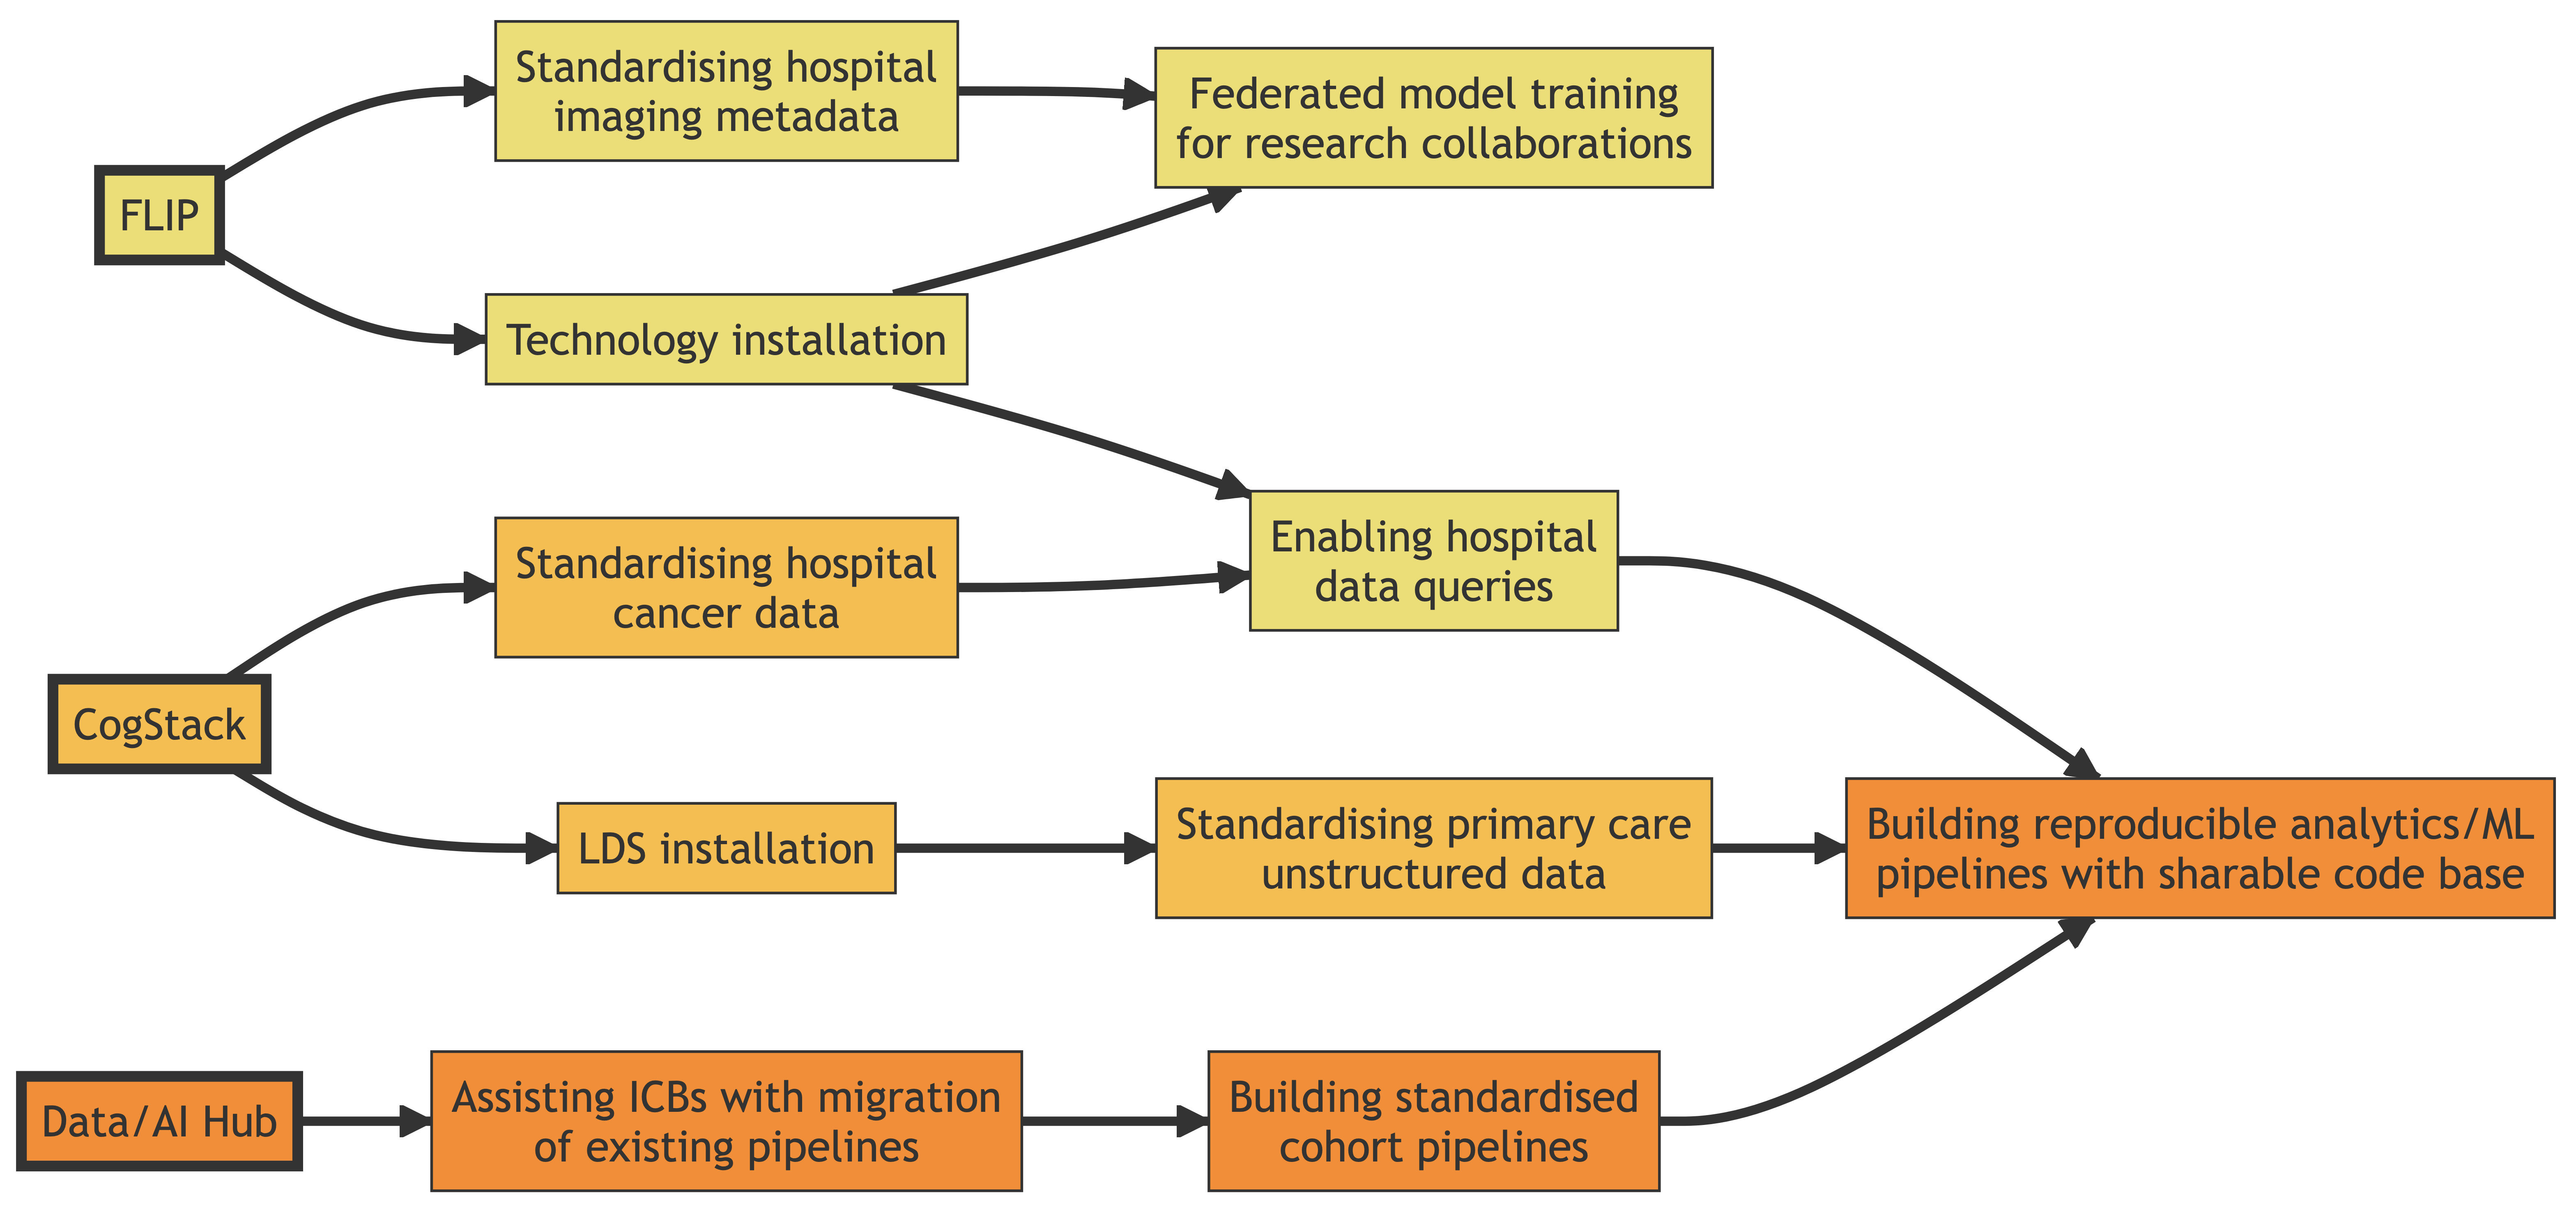
\includegraphics[width=6in,height=4.27in]{index_files/figure-latex/mermaid-figure-6.png}

}

\caption{\label{fig-sde-summary}Summary of SDE components and data
flows. Each London ICB is provisioned with its own data/analytics
environment through the LDS. FLIP = Federated Learning and
Interoperability Platform.}

\end{figure}%

\textsubscript{Source:
\href{https://d3london.github.io/sde_aic_docs/index.qmd.html}{Article
Notebook}}

\subsection{Technology and objectives}\label{technology-and-objectives}

The contribution from the London AIC consists of technology deployment
and supporting expertise, that enable a number of objectives
(Figure~\ref{fig-aic-objectives}) over the two year programme. This
contribution includes the following:

\begin{enumerate}
\def\labelenumi{(\arabic{enumi})}
\item
  \textbf{Federated Learning and Interoperability Platform (FLIP)}: FLIP
  consists of (a) secure data environments within NHS hospital Trusts
  for multi-modal imaging data, imaging metadata, and structured health
  record data in the OMOP common data model; and (b) a mechanism to
  query data and train AI models across these secure enclaves without
  the need to physically transfer data. FLIP is presently installed in
  four major London Trusts. Integrating FLIP into the SDE will enable
  hospital data (such as cancer data) to be surfaced into the LDS, and
  enable access to multi-modal data (such as DICOM imaging and digital
  pathology) for research in precision medicine.
\item
  \textbf{CogStack}: As an advanced natural language processing
  platform, CogStack can turn the large quantities of health information
  that are found in narrative text, into structured and analysable data.
  Currently actively used in Trusts to assist with clinical coding from
  notes and clinic letters, CogStack can surface secondary care and
  cancer pathway data, and previously unseen primary care data, into the
  SDE ecosystem.
\item
  \textbf{AIC Data/AI Hub}: The AIC hosts health data and AI
  implementation expertise, that will provide practical support in
  analytics engineering, clinical informatics, data science, and machine
  learning (ML) development and deployment. Primary aims are to (a) help
  Integrated Care Boards (ICB) migrate data pipelines and analytics into
  common data models and terminologies within LDS environments; (b)
  extend these into reproducible pipelines for data science and
  predictive analytics deployment; and (c) work together to make ICBs
  self-sufficient in these capabilities. The AIC will also support the
  adoption and roll-out of the OMOP Common Data Model.
\end{enumerate}

\begin{figure}

\centering{

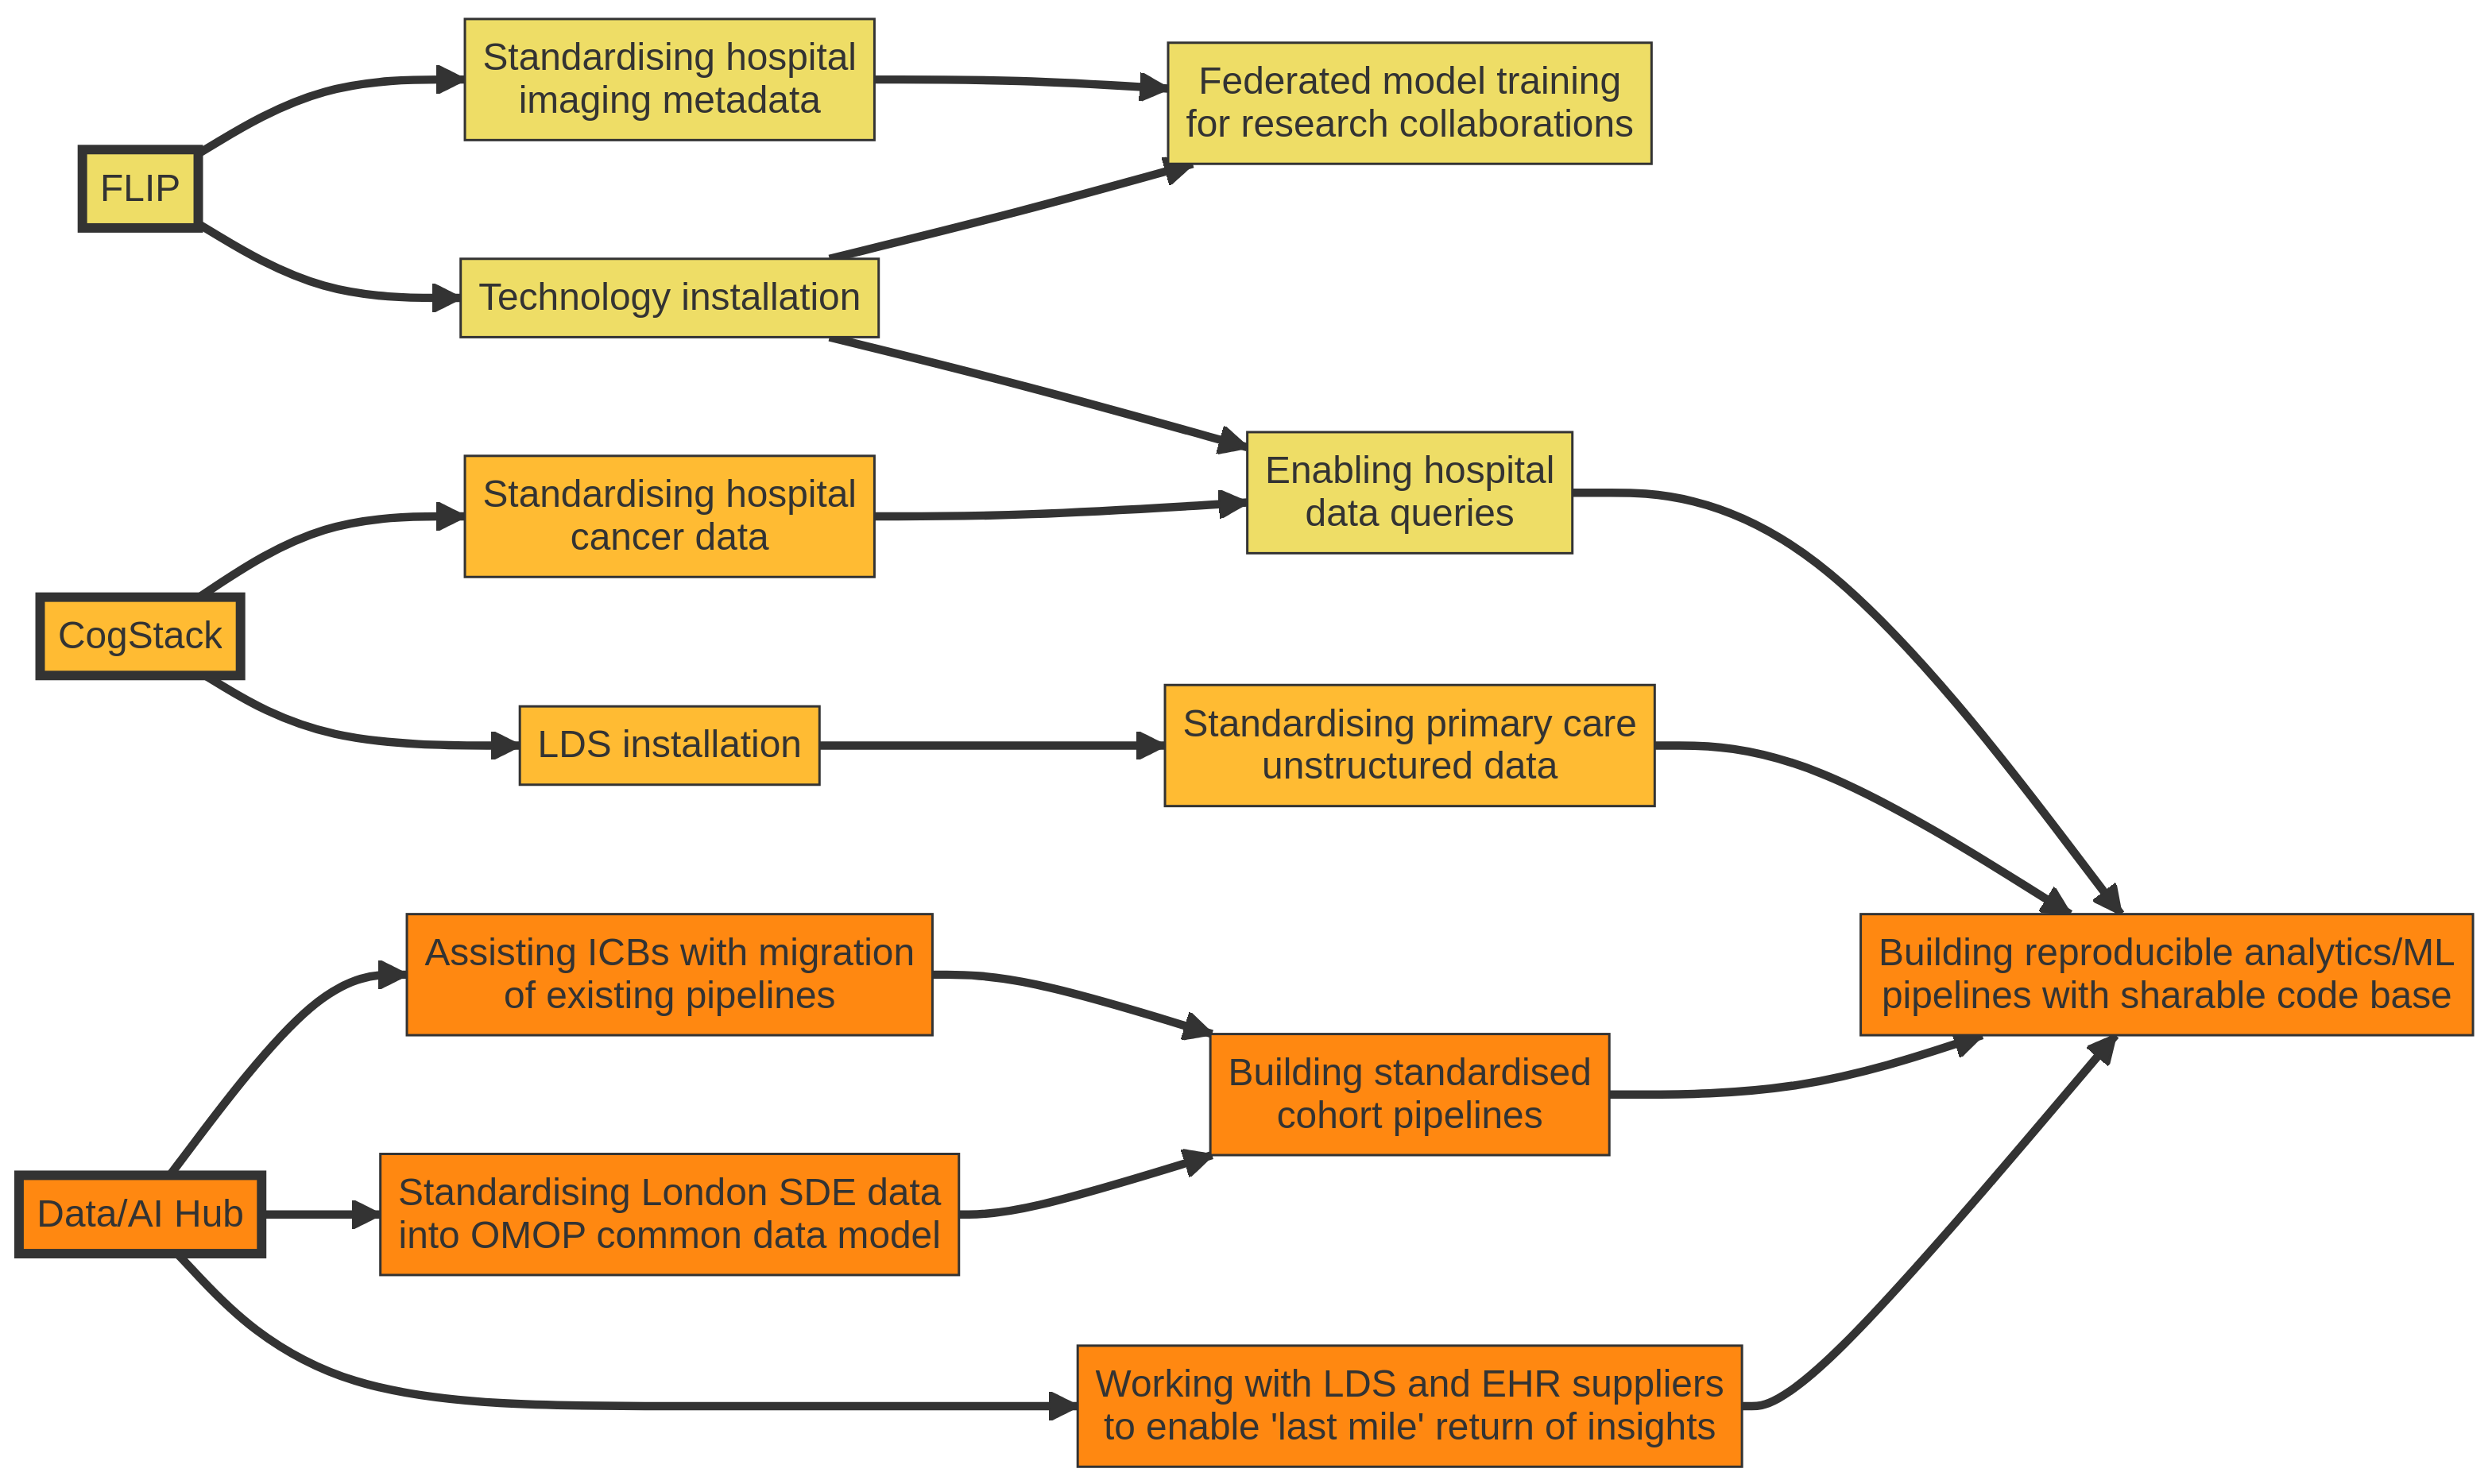
\includegraphics[width=6in,height=3.58in]{index_files/figure-latex/mermaid-figure-10.png}

}

\caption{\label{fig-aic-objectives}Summary of AIC work components and
objectives. FLIP = Federated Learning and Interoperability Platform; ML
= Machine Learning; EHR = Electronic Health Record}

\end{figure}%

\textsubscript{Source:
\href{https://d3london.github.io/sde_aic_docs/index.qmd.html}{Article
Notebook}}

As the LDS ICB environments share a common data model, any pipelines
created in collaboration with one ICB can be adapted and used for any
other ICB (or deployed across multiple environments to create pan-London
insights). This will also facilitate the use of shared terminologies,
and validating / versioning / serving NHS-owned machine learning models
across regions.

\subsection{Proposed use-cases}\label{proposed-use-cases}

The following three use-cases are \emph{examples} of analytics projects
that can be supported within the SDE ecosystem, in collaboration between
ICB/NHS analytics teams and the AIC/SDE team. Use-cases align to the
London Health Data Strategy and long term condition priorities, as well
as national programmes such as CORE20PLUS5, and are proposed here
following early discussions with London ICBs. An objective for any work
is to build upwards from a foundation of reproducible pipelines, towards
data science and predictive analytics
(Figure~\ref{fig-general-framework}).

\begin{figure}

\centering{

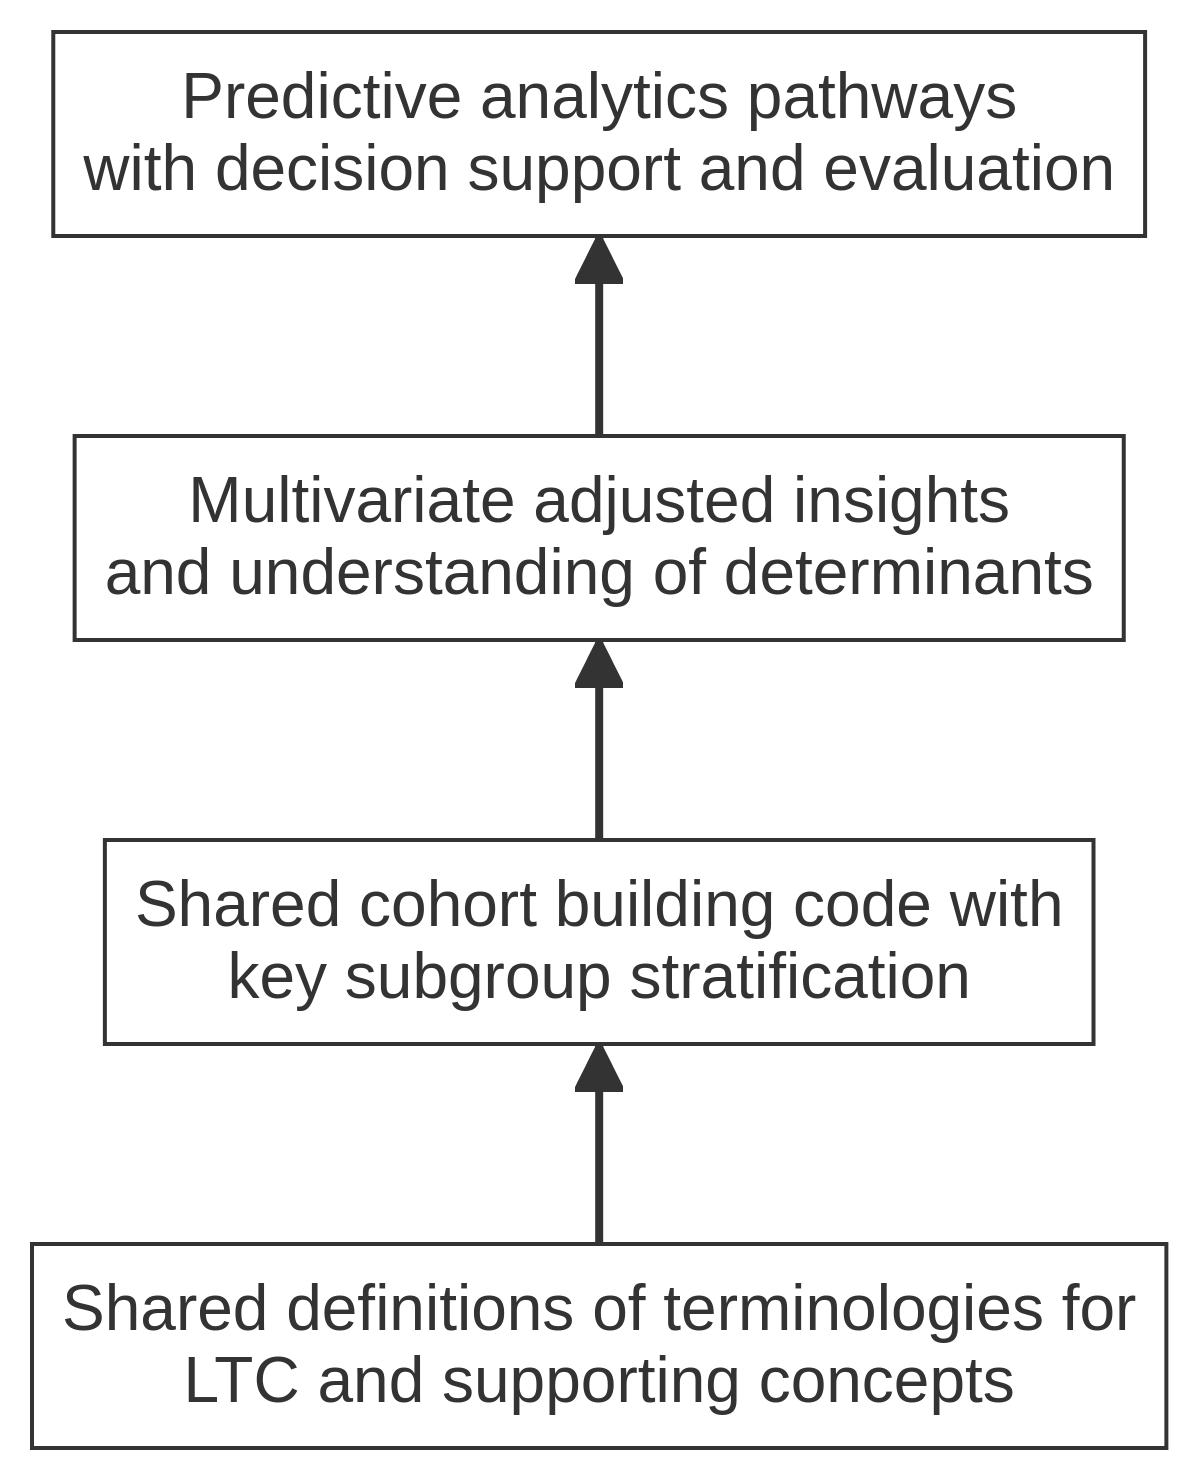
\includegraphics[width=6in,height=7.41in]{index_files/figure-latex/mermaid-figure-9.png}

}

\caption{\label{fig-general-framework}General framework for use-cases:
moving towards advanced analytics}

\end{figure}%

\textsubscript{Source:
\href{https://d3london.github.io/sde_aic_docs/index.qmd.html}{Article
Notebook}}

\subsubsection{Systematic measurement of group and individual health
inequality}\label{systematic-measurement-of-group-and-individual-health-inequality}

\textbf{AIM:} To systematically surface multiple dimensions of health
inequality across sociodemographic / geospatial groups, and across
individual patients, and to monitor this data continuously across key
long-term conditions.

\textbf{SUMMARY:} Health inequality refers to differences in health
outcomes and determinants between individuals or groups (e.g.~morbidity,
co-morbidity, disease complications/death, healthcare access, disease
screening, treatment delivery). The principle of health \emph{equity}
emphasises the recognition and reduction of disparities in determinants,
resulting in more equal outcomes.

It is important to understand what groups suffer from health inequality.
This is traditionally measured and visualised as a comparison of disease
and outcome prevalence/incidence across different population groups.
While helpful for broad insights, this also offers limited understanding
of complex individual circumstances and determinants. This use-case
proposes that measurement of inequalities can be extended to individual
patients, by using clinical domain knowledge to define `indicators' of
unequal disease, diagnosis, and treatment pathways. In an individual
with a long-term condition (LTC), example indicators of inequality are
shown below. The contribution of individual indicators to later outcomes
can also be measured in multivariate statistical models, and used to
understand determinants for any given individual.

\begin{longtable}[]{@{}
  >{\raggedright\arraybackslash}p{(\columnwidth - 0\tabcolsep) * \real{1.0000}}@{}}
\toprule\noalign{}
\endhead
\bottomrule\noalign{}
\endlastfoot
1. LTC surfacing at an early age (Figure~\ref{fig-onset-time}) \\
2. LTC in proximity to relevant co-morbidities (e.g.~cardiovascular risk
factors) \\
3. Diagnosis at a \emph{late} age but with more severe disease (e.g.~in
Diabetes, measured by HbA1c or presence of end-organ complications) \\
4. Reduced health engagement/encounters/treatment compared to what is
expected based on disease severity \\
5. Shorter time to complications and mortality following diagnosis \\
\end{longtable}

The objective is to move beyond describing inequality, to understanding
individual/small group determinants, and to increase actionability. At
this level, determinants can be visualised for small specific groups, or
individuals, with comparison to `what is expected' in a background
population.

\begin{figure}

\centering{

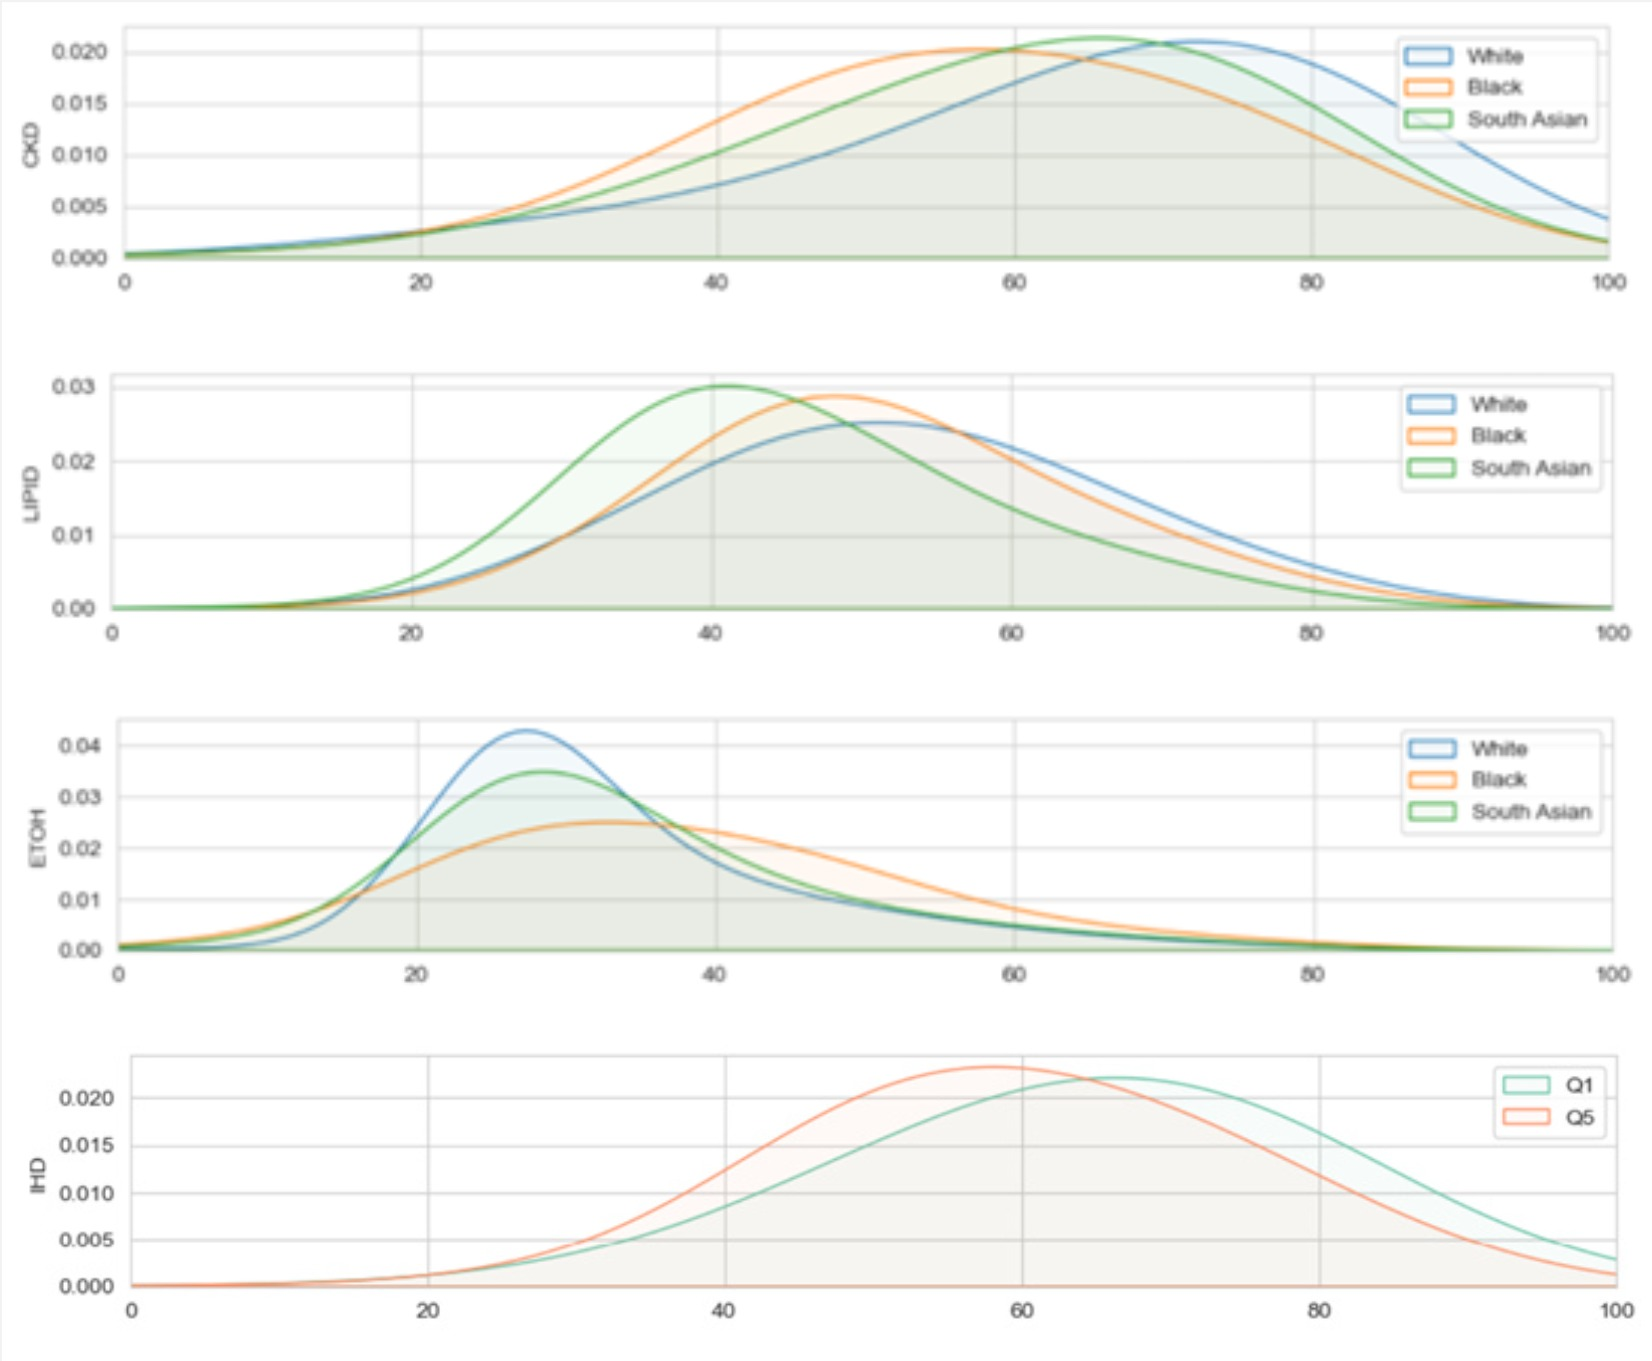
\includegraphics{media/onset_over_time.jpg}

}

\caption{\label{fig-onset-time}Inequality in age of onset across
demographic groups and deprivation, generated automatically through
input of condition and group for stratification}

\end{figure}%

As per the framework described in (Figure~\ref{fig-general-framework}),
the initial stage of work will include defining shared terminologies,
concepts, and indicators that cover LTC of interest. Secondly, existing
descriptions of health inequality can be migrated onto the LDS
environment, and extended such that any condition can be reproducibly
visualised across multiple dimensions and `cuts'. This foundation can be
further extended to encompass specific inequality indicators and
statistical insights, at a small group and individual level, and the use
of these insights to identify patients at greatest risk of health
inequality, or those with addressable determinants.

\subsubsection{Cardiovascular disease prevention through decision
intelligence}\label{cardiovascular-disease-prevention-through-decision-intelligence}

\textbf{AIM:} To enhance descriptive population health management with
explainable predictive analytics and clinical guideline-based ``decision
intelligence'' systems, across cardiovascular related co-morbidities
(including hypertension, diabetes, chronic kidney disease).

\textbf{SUMMARY:} The spectrum of cardiovascular long-term conditions
(LTC) and associated risk factors is wide, and includes hypertension,
diabetes, obesity, high cholesterol, ischaemic heart disease, stroke,
and chronic kidney disease, as well as dementia, atrial fibrillation,
and heart failure. The burden of such diseases is high.
\href{https://cks.nice.org.uk/topics/cvd-risk-assessment-management/background-information/burden-of-cvd/}{Heart
disease} alone causes a quarter of deaths in the UK, with direct costs
to the healthcare system estimated at £9 billion by the British Heart
Foundation. Cardiovascular disease is seen as a
\href{https://imperialcollegehealthpartners.com/portfolio/onelondon/}{priority
area for use of data} across OneLondon patient and public engagement.

\begin{figure}

\centering{

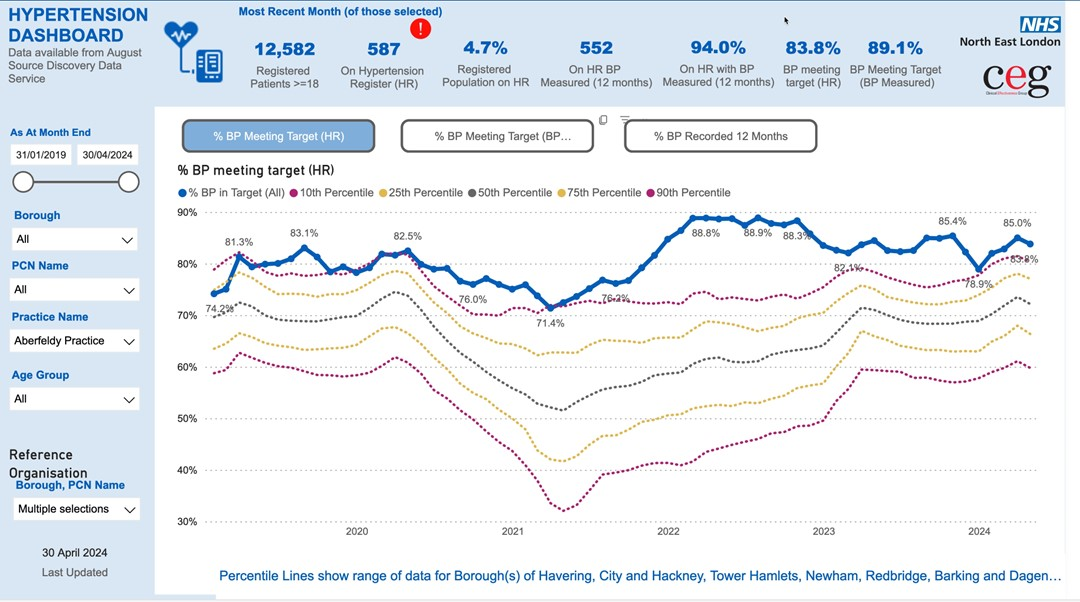
\includegraphics{media/example_dashboard.jpg}

}

\caption{\label{fig-icb-hypertension}Existing ICB dashboard for
Hypertension}

\end{figure}%

In London ICBs, there is robust aggregate understanding of LTC, through
prevalence reporting and Quality Outcome Framework (QOF) indicators.
Existing ICB dashboards (Figure~\ref{fig-icb-hypertension}) show how a
practice or a system are performing relative to their peers. However,
such reporting has limitations, including: (1) lack of adjustment for
demographics and other confounding variables; (2) difficulty in
surfacing individual patients with direct actions; and (3) lack of
consideration of complex co-morbidity phenotypes. This last is
particularly important, as multi-morbidity changes the risk profile and
urgency of response for individuals. Some of these limitations are being
addressed by existing work in London pathfinder programmes, and in other
regions such as Greater Manchester, which are moving towards electronic
identification of patients who may be actioned via pre-agreed clinical
pathways (Figure~\ref{fig-simple-pathway-action}).

\begin{figure}

\centering{

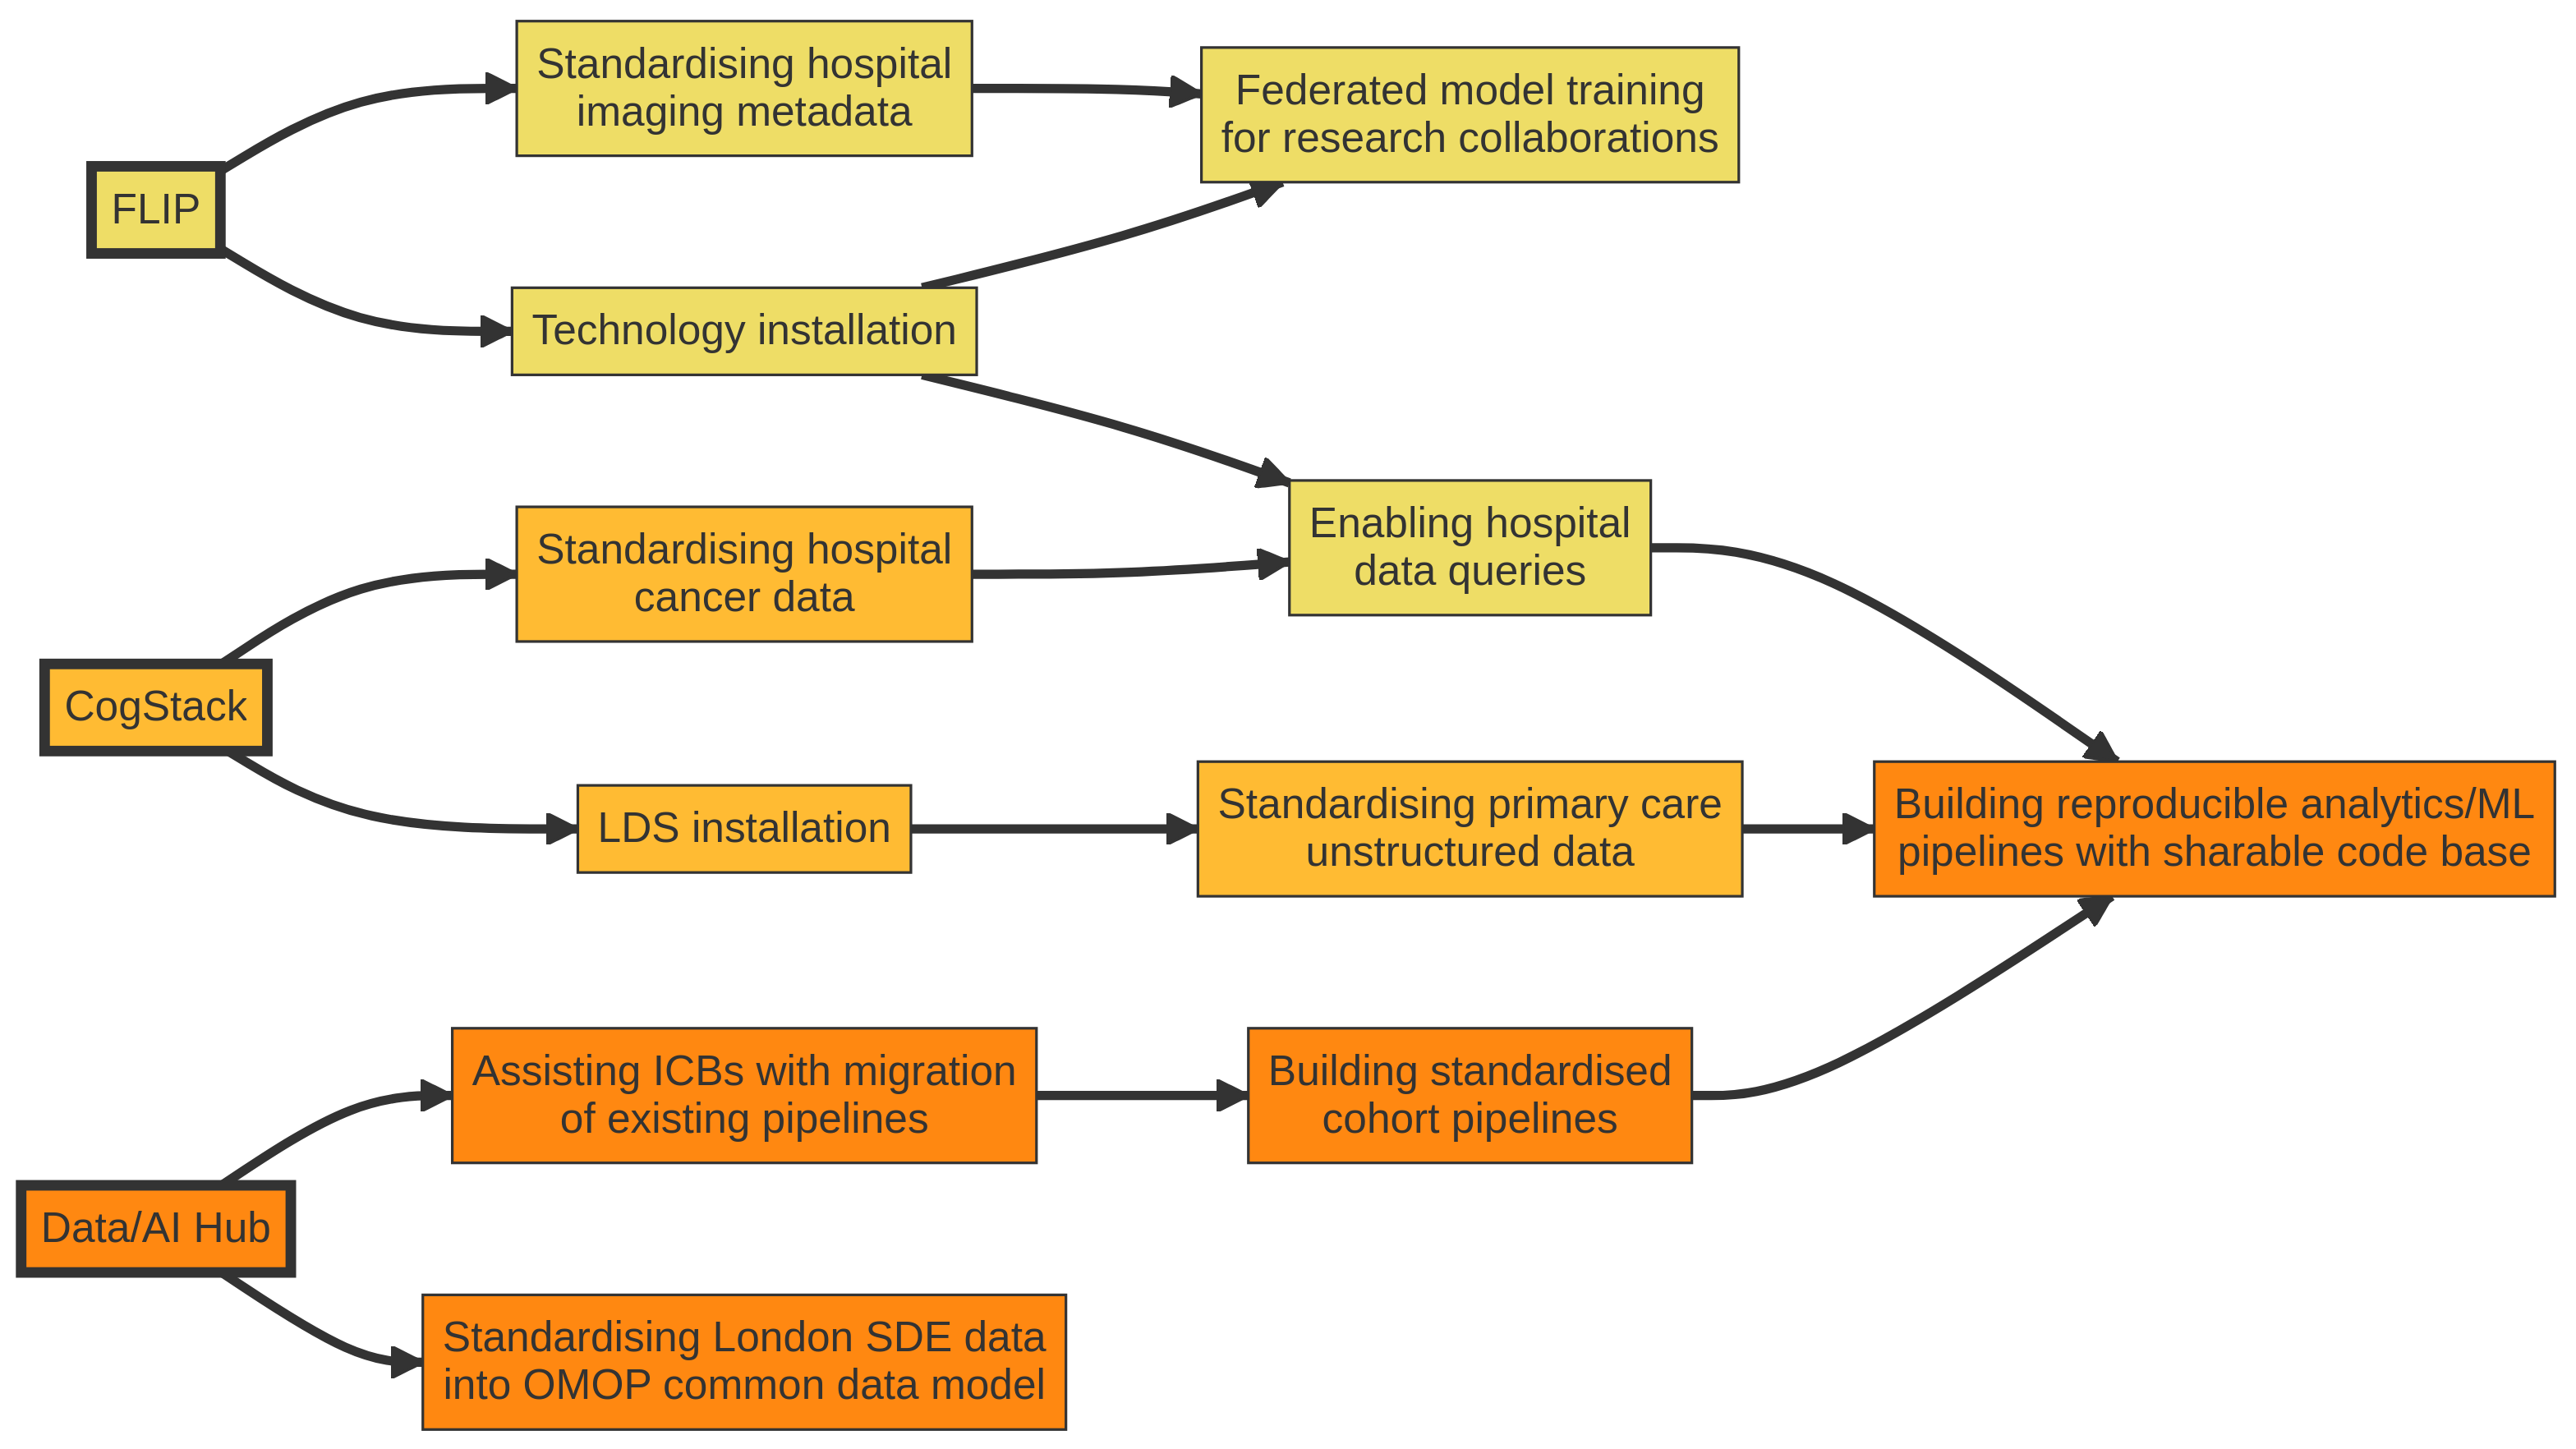
\includegraphics[width=6in,height=2.51in]{index_files/figure-latex/mermaid-figure-8.png}

}

\caption{\label{fig-simple-pathway-action}Examples of simple logical
triggers leading to clinical actions. CKD = Chronic Kidney Disease; BB =
Beta-blocker; ACEi = ACE inhibitor.}

\end{figure}%

\textsubscript{Source:
\href{https://d3london.github.io/sde_aic_docs/index.qmd.html}{Article
Notebook}}

These limitations can be surmounted through using richer data to
generate personalised risk profiles for individual patients (rather than
aggregate group summaries). A previous collaboration between the AIC and
North-East London ICB was able to develop precise cardiovascular risk
prediction models for individuals, using explainable machine learning
algorithms and the linked patient health record. Actionable factors
could also be highlighted in patients with high risk, with their
relative importance explained through statistical modelling to enhance
explainability (Figure~\ref{fig-htn-actionable}).

\begin{figure}

\centering{

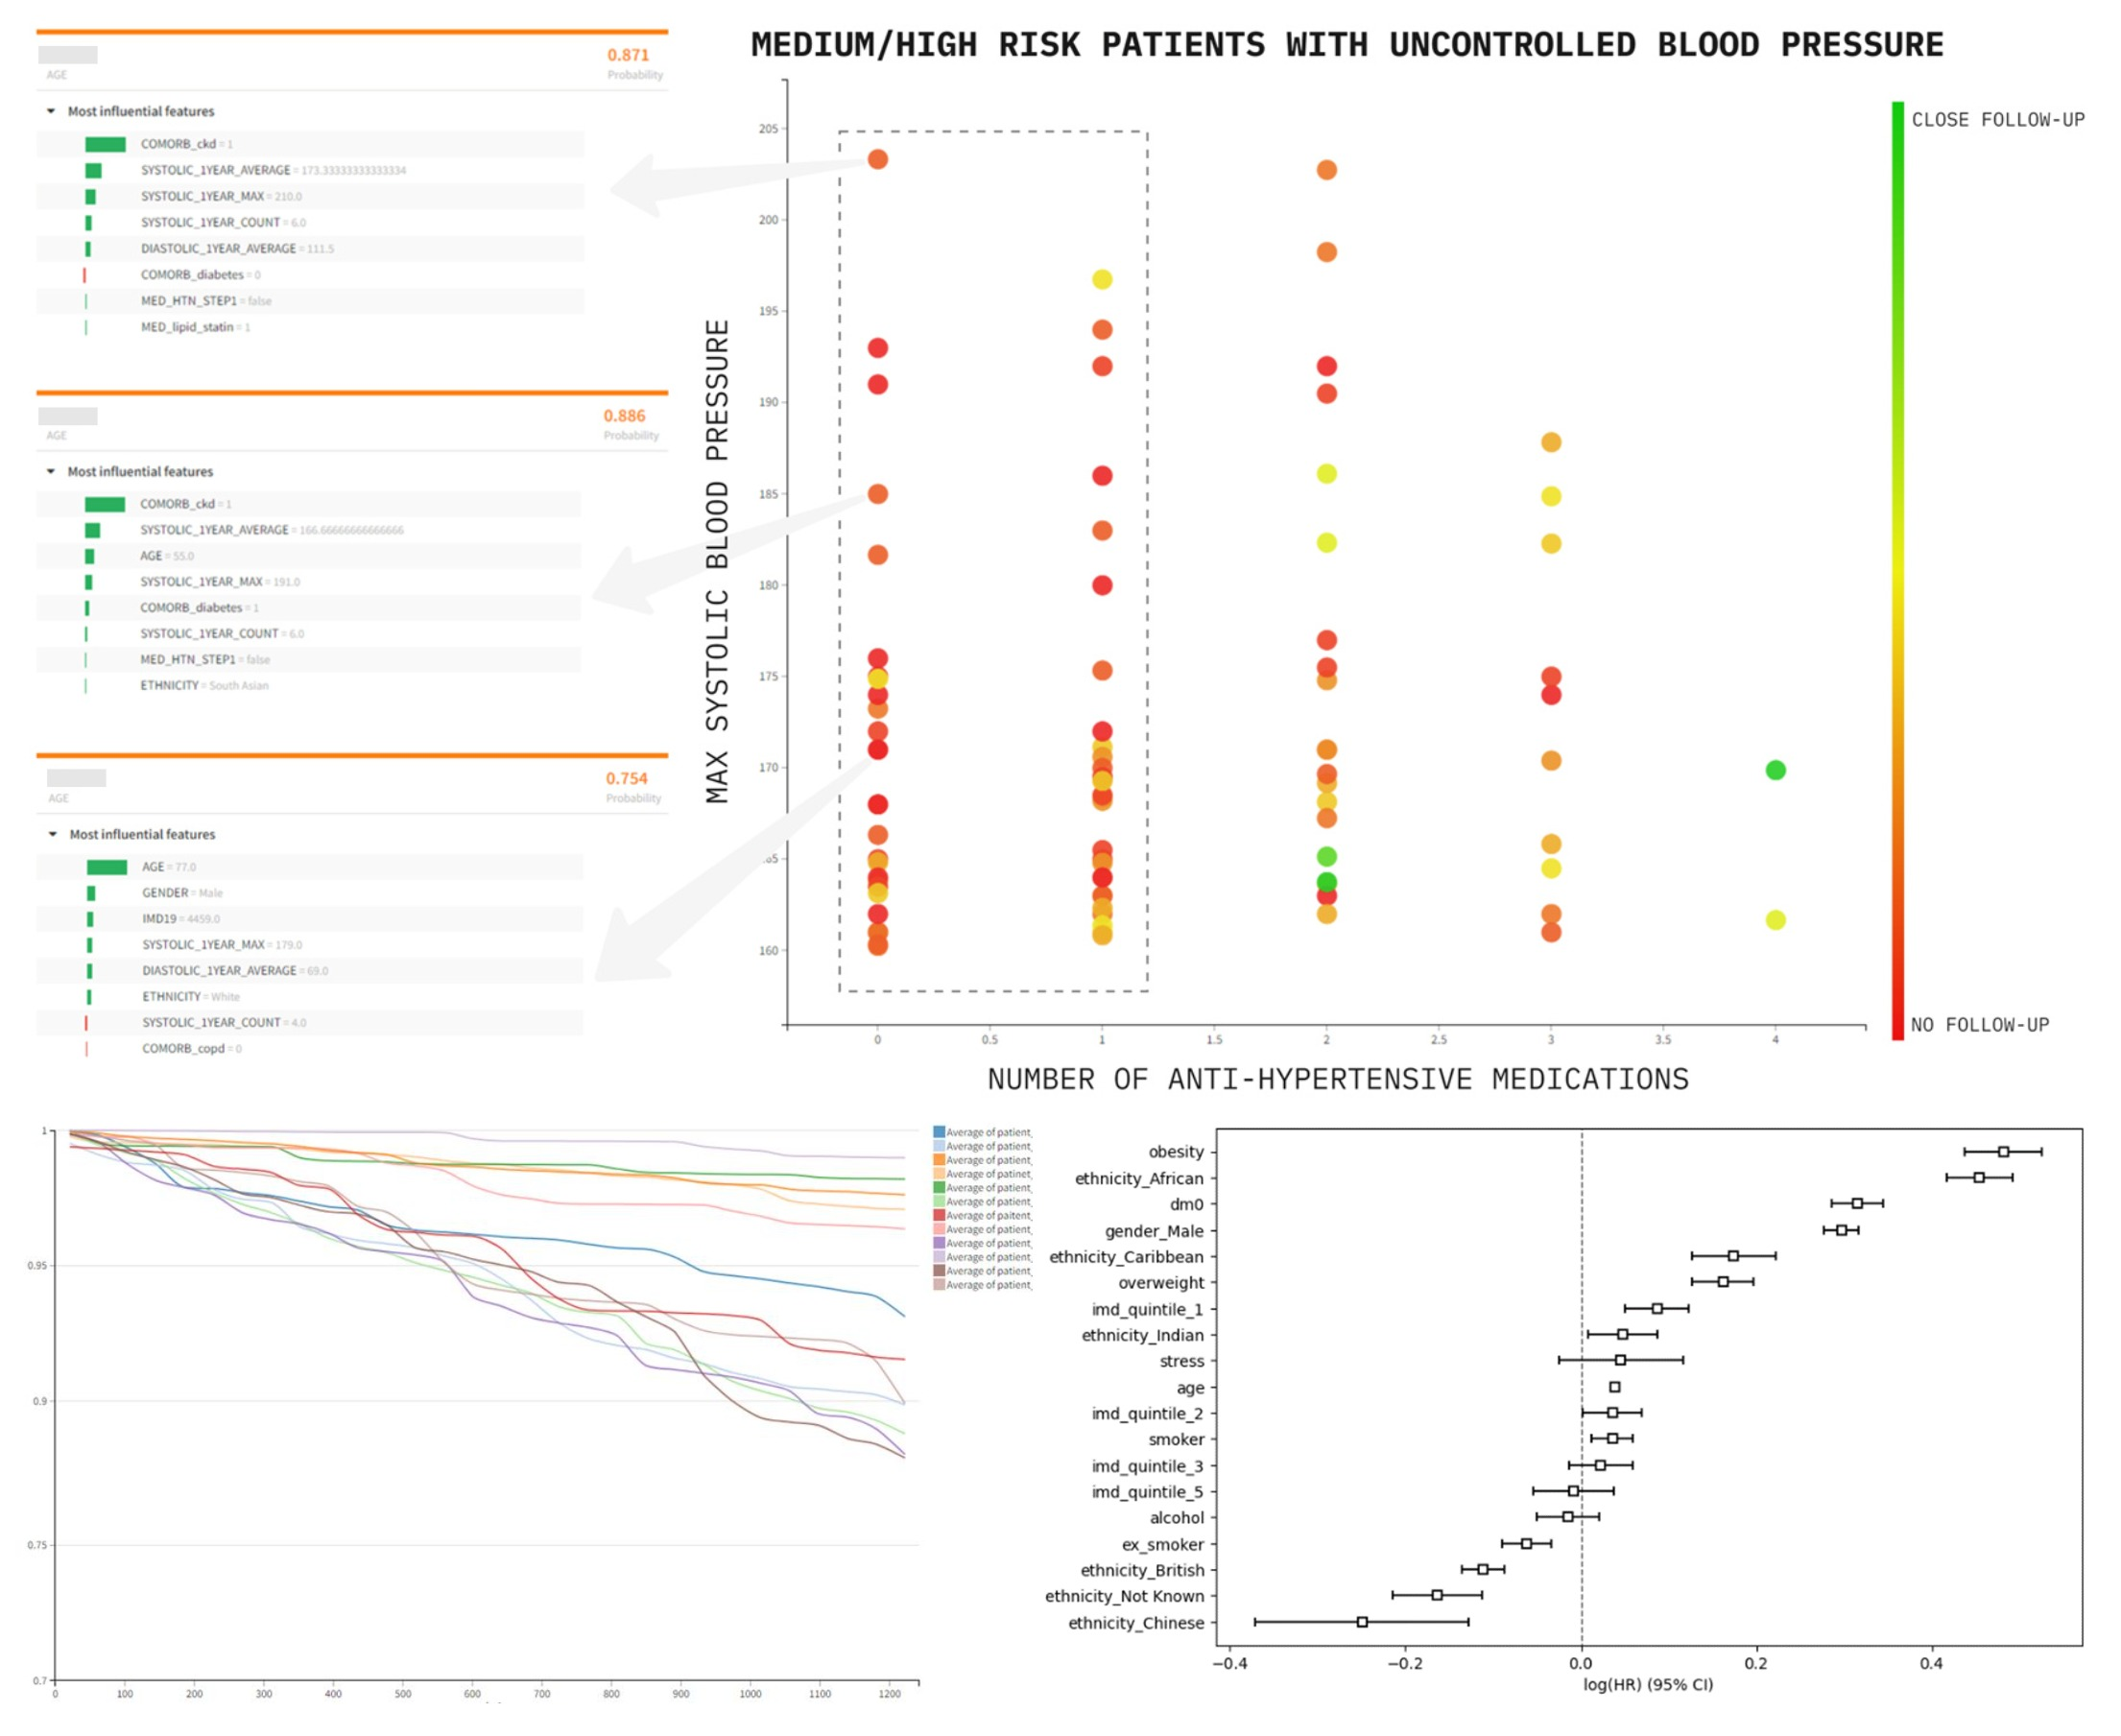
\includegraphics{media/htn_actionable.jpg}

}

\caption{\label{fig-htn-actionable}Actionable factors (including
follow-up, treatment, blood pressure control) and association of
features with adverse outcome in high risk hypertensive patients}

\end{figure}%

Predictive analytics alone are not a solution. Patients identified as
``high risk'' may have few clinical factors that can be optimised, and
non-specific risk stratification is known to lead to
\href{https://bmjopen.bmj.com/content/9/6/e026470}{increased resource
utilisation without improving outcomes}. Instead, this use-case proposes
the use of validated clinical guidelines and domain knowledge to
identify specific optimisation or preventative actions - much like
Figure~\ref{fig-simple-pathway-action}, but systematically, and on a
larger scale. The combination of predictive analytics and explicitly
defined actions to support decisions, is known as
\href{https://www.gartner.com/en/information-technology/glossary/decision-intelligence}{``decision
intelligence''}.

This use-case will again first develop shared terminologies, features,
and code to enhance current pipelines and dashboards
(Figure~\ref{fig-general-framework}). This is an opportunity for using
new programme capabiltiies to extend existing work through:

\begin{longtable}[]{@{}
  >{\raggedright\arraybackslash}p{(\columnwidth - 0\tabcolsep) * \real{1.0000}}@{}}
\toprule\noalign{}
\endhead
\bottomrule\noalign{}
\endlastfoot
(1) Using CogStack to extract additional valuable context and missing
codes from unstructured text to improve performance, and reduce
potential for negative biases, in predictive models; \\
(2) Computerising Quality Outcomes Framework targets and clinical
guidelines, in conjunction with local clinical teams, to develop safe
decision logic for use as part of an effector arm; \\
(3) Using rich features in the EHR to develop statistical and machine
learning models for predicting and understanding risk of progression and
acute care utilisation across cardiovascular morbidity and
co-morbidity; \\
(4) For a given patient's health record, understanding actions (i.e.~are
there actions available, and what are they), combined with explainable
risks across multiple conditions (i.e.~what are the highest risks for
this patient and why), to support decision-making; \\
(5) Returning individual patient insights and suggested actions to
clinical systems such as EHR (EMIS) or the London Care Record \\
\end{longtable}

Highly individualised patient profiles are the objective of personalised
care, and are a key component of preventative healthcare. Any deployed
systems will need to be evaluated and monitored for safety and fairness,
with a process of training and handover to continuity teams following
the end of this SDE programme phase. This is the objective of on-going
work by responsible AI and AI governance teams in the AI Centre.

\subsubsection{Joining up cancer
pathways}\label{joining-up-cancer-pathways}

\textbf{AIM:} To link cancer pathways (including screening, diagnosis,
staging, and outcomes) across primary care and secondary care. To
identify areas of inequality in screening and late diagnosis, and to
generate predictive insights for risk and screening recall.

\textbf{SUMMARY:} Cancer has long been a challenging area for
data-driven initiatives. Primary care coding of cancer is often
incomplete, as the majority of care following referral takes place in
hospitals. The most readily available secondary care data is from
Commissioning Data Sets, which are only complete for inpatient care, and
may not include the majority of cancer events. Within hospitals, the
largest quantity of cancer data sits within audit datasets, or within
unstructured text and clinic letters, which are not easily accessible.

This results in significant limitations. First, it is difficult to
reconcile screening data with diagnostic outcomes. Second, only an
incomplete picture of cancer diagnoses can be obtained at the ICB level,
including of disease severity following delayed referral or prolonged
waiting time. Finally, it is difficult to gain understanding of how such
pathways impact on overall treatment outcomes and cancer recurrence.

The SDE programme provides opportunities to surface and link currently
missing data, to provide an end-to-end overview of key cancer pathways.
Figure~\ref{fig-sde-summary} has been adapted below to show cancer data
flows within the SDE ecosystem (Figure~\ref{fig-cancer-data}). This work
is complementary to additional work with FLIP to make cancer imaging and
digital pathology data available, to support precision medicine research
in the same patient cohorts.

\begin{figure}

\centering{

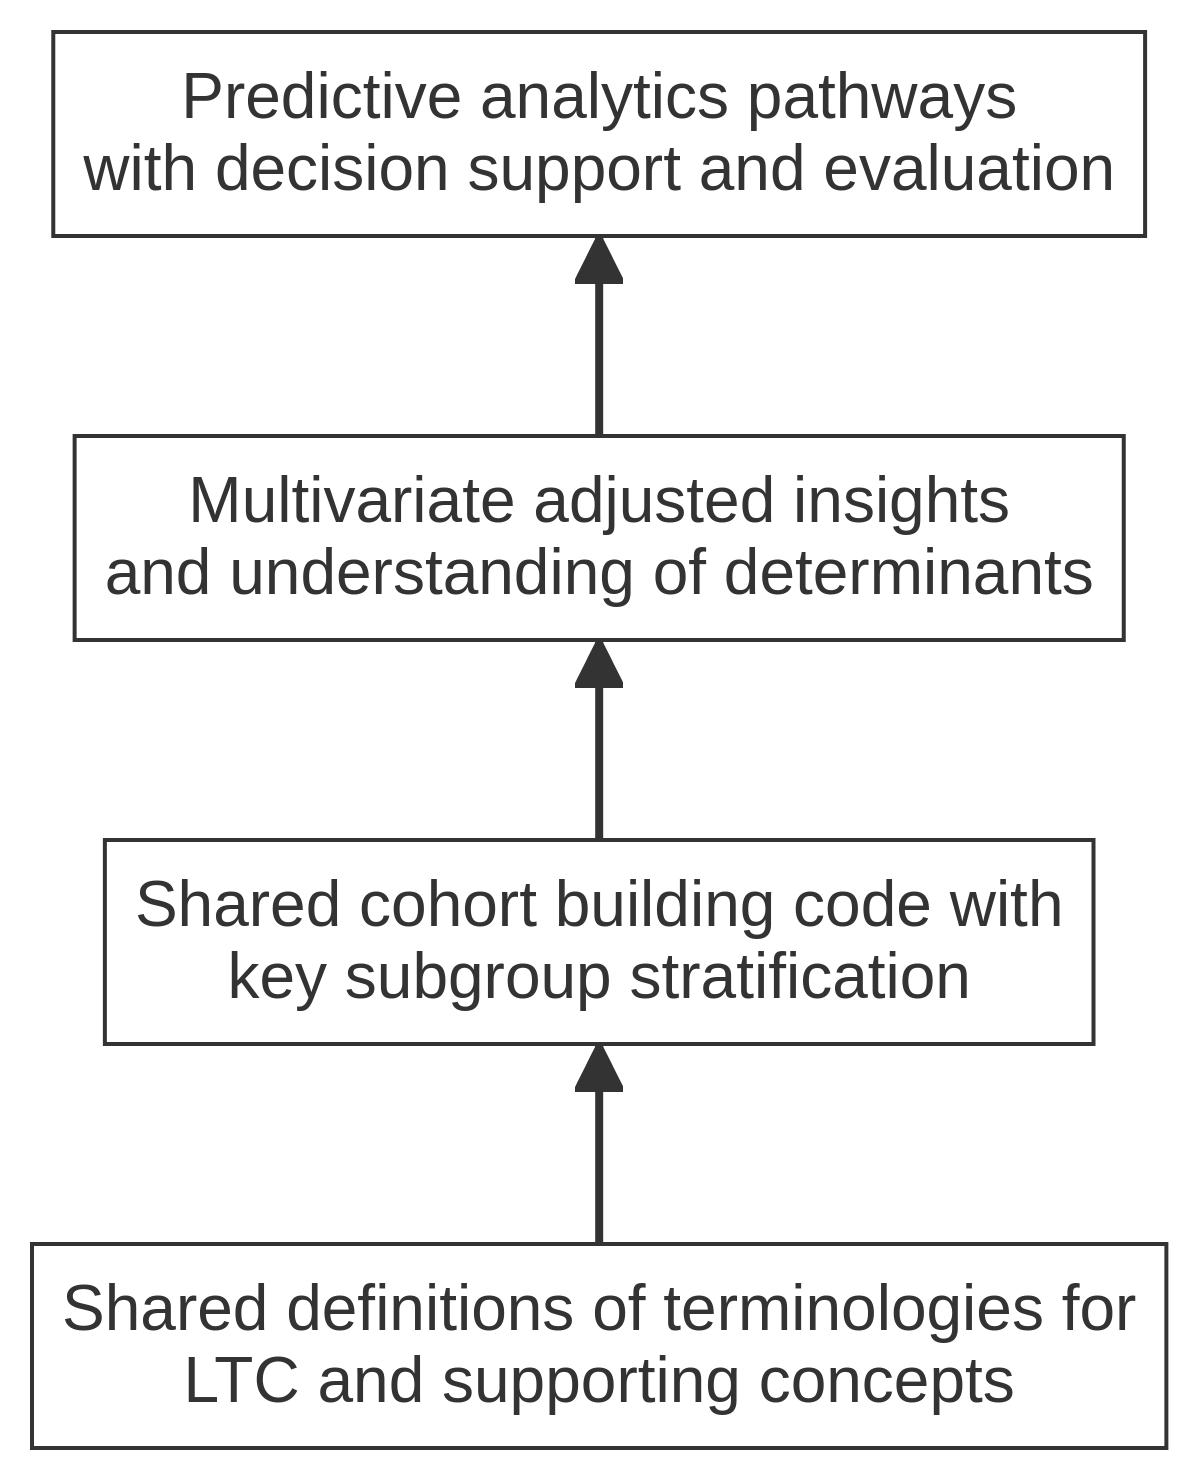
\includegraphics[width=6in,height=4.98in]{index_files/figure-latex/mermaid-figure-7.png}

}

\caption{\label{fig-cancer-data}Summary of cancer data flows within the
London SDE ecosystem.}

\end{figure}%

\textsubscript{Source:
\href{https://d3london.github.io/sde_aic_docs/index.qmd.html}{Article
Notebook}}

It is expected that year one of the programme will consist of
infrastructural work to enable these data flows, with a focus on two
cancer areas, \textbf{breast cancer} and \textbf{lung cancer}. This work
will include the installation of technology such as CogStack and FLIP,
and creating pipelines to standardise data into OMOP to enable linked
querying and federated analytics. Year two will enable a number of
analyses for each cancer area that can support understanding of
population health, health inequalities, and pathway bottlenecks, and
ultimately support the use of predictive analytics to address late
referrals, missed screening, and late diagnosis.

\begin{longtable}[]{@{}
  >{\raggedright\arraybackslash}p{(\columnwidth - 0\tabcolsep) * \real{1.0000}}@{}}
\toprule\noalign{}
\endhead
\bottomrule\noalign{}
\endlastfoot
(1) How common is later stage cancer diagnosis following primary care
referral, and what is the incidence/prevalence of late diagnosis across
different patient groups and geographies? \\
(2) Which patient groups are most subject to screening delay or refusal,
and what is the impact on late cancer diagnoses? \\
(3) In a typical longitudinal cancer ``journey'' (including screening/GP
presentation with symptoms -\textgreater{} referral/investigation
-\textgreater{} diagnosis -\textgreater{} treatment initation), where
are the major delays? Is there inequality in how patient groups are
affected by delays? \\
(4) Can the unstructured and structured GP record be used to inform
cancer risk and referrals through predictive analytics? \\
(5) Can population groups with cancer outcomes inequality be targeted to
increase early diagnosis rates? \\
\end{longtable}

Ultimately, a major aim of this SDE programme phase is to bring cancer
data availability, linkage, and utilisation in line with other long-term
conditions, and to enable systematic evaluation across the entire cancer
pathway.

\subsection{Next steps}\label{next-steps}

This phase of the London SDE programme commenced in April 2024, along
the roadmap described in Figure~\ref{fig-aic-objectives}. With each ICB
having their own requirements, objectives, and timelines, the AIC
Data/AI Hub has been commissioned to support `as much' or `as little' as
required: initially to help with standardisation of terminologies and
cohort definitions, and eventually to help create a code base and model
library that can be shared and re-used across the London region. It is
also the intention to help pass on specific technical expertise and
other practices to ICB teams, to enable continuity following the end of
the programme.



\end{document}
